% small.tex
\documentclass[12pt]{beamer}
\usetheme{amcg}
\beamertemplatenavigationsymbolsempty
\renewcommand{\thefootnote}{}
\providecommand{\e}[1]{\ensuremath{\times 10^{#1}}}
\usepackage{amsmath}
\usepackage{bm}
\usepackage{mathptmx}
\usepackage{helvet}
\usepackage{cancel}
\newcommand\TILDE{\char`\~}
\usepackage{listings}
\usepackage[absolute,overlay]{textpos}
\setlength{\TPHorizModule}{\textwidth} % Horizontale Einheit
\setlength{\TPVertModule}{\textheight} % Vertikale Einheit
\usepackage[latin1]{inputenc}
\usepackage{tikz}
\usetikzlibrary{shapes,arrows,backgrounds,fit,shadows,positioning}
\usepackage{natbib}
% beamer+natbib is not supported, so we need this hack
\def\newblock{\beamer@newblock}

% items enclosed in square brackets are optional
\title[Numerics]{Numerical considerations when configuring Fluidity}
\subtitle[]{}
\institute{Applied Modelling and Computation Group\\
Department of Earth Science and Engineering\\
Imperial College London}
\author[Stephan Kramer]{Stephan Kramer}
\date{}

\newcommand\pp[2]{\frac{\partial #1}{\partial #2}}
\newcommand\ppt[1]{\pp{#1}t}
\newcommand\grad\nabla
\renewcommand\div{\nabla\cdot}

\newcommand\mat[1]{\mathrm{#1}}

\newcommand\dv[1]{\underline{\bf #1}} % discrete vector
\newcommand\vT{\dv T}
\newcommand\vu{\dv u}
\newcommand\vf{\dv f}
\newcommand\vp{\dv P'}

\newcommand\poo{P1-P1}
\newcommand\podgpt{P1$_{\text{DG}}$-P2}
\renewcommand\emph[1]{{\bf #1}}
\begin{document}

% This little snippet adds the outline slide with the
% current section highlighted between each section
\AtBeginSection[]
{
   \begin{frame}
       \frametitle{Outline}
       \tableofcontents[currentsection]
   \end{frame}
}

%--- the titlepage frame -------------------------%
\begin{frame}
  \titlepage
\end{frame}

%-- Overview slide --- %
\section*{Outline}
\begin{frame}
  \frametitle{Outline}
  \tableofcontents
\end{frame}

%-- Add sections and your outline will be created automatically --%
\section{Time integration}

\begin{frame}{Time integration}
  Consider the advection diffusion equation:
  \begin{equation*}
    \ppt T + \vec u\cdot\grad T - \kappa \nabla^2 T = 0.
  \end{equation*}
  After finite element discretisation, we obtain a semi-discrete equation:
  \begin{equation*}
    \mat M\ppt \vT + \mat A(\vec u) \vT + \mat D \vT = 0.
  \end{equation*}
  which is an ODE in matrix form for the solution vector $\vT$ with
  time-dependent coefficients. The finite element method tells us how to
  assemble the mass matrix $\mat M$, the advection matrix $\mat A(\vec u)$ and
  diffusion matrix $\mat D$.
\end{frame}

\begin{frame}{Explicit Euler\hspace{10ex}.}
  \begin{textblock}{0.3}(.8,0)
     \includegraphics[width=\textwidth]{forward-euler.png}
  \end{textblock}
  \begin{minipage}{0.7\textwidth}
  Time integration with the  explicit \\
  \emph{forward Euler} time stepping method:
  \begin{equation*}
    \mat M\frac{\vT^{n+1}-\vT^n}{\Delta t} 
    + \mat A(\vec u) \vT^n + \mat D \vT^n = 0
  \end{equation*}
  or
  \begin{equation*}
    \mat M \vT^{n+1} = \mat M \vT^n - \Delta t \left(
    \mat A(\vec u) \vT^n + \mat D \vT^n \right)
  \end{equation*}
\end{minipage}

  \only<1>{
    \vspace{1ex}
  Even for an explicit method we still end up with a matrix equation to solve!
  For Continuous Galerkin FEM the inverse mass matrix is dense.
  In some cases we approximate the mass matrix by a diagonal matrix
  in a process called \emph{mass lumping}.}
  \only<2>{
  \begin{block}{Courant condition}
    The explicit method is only \emph{conditionally} stable. For advection,
    a Courant
    condition applies similar to that for finite differences:
    \begin{equation*}
      \frac{u \Delta t}{\Delta x} < 1
    \end{equation*}
  \end{block}}
\end{frame}

\begin{frame}{Courant condition \& unstructured}
  Courant condition depends on numerical scheme.
  \begin{example}
    \small
    \begin{minipage}{0.7\textwidth}
      Consider first--order--upwind finite volume for advection
      of a concentration $c$. For simplicity, assume that the
      volume fluxes, normal velocity $u_n$ times width $w$,
      in and out of cell 2 are equal (i.e.
      incompressible flow). For cell 2 with area $A_2$, we have:
      \begin{equation*}
        A_2 c^{n+1}_2 = A_2 c^n_2 + \Delta t \left(u_n w c^n_1-u_n w c^n_2\right)
      \end{equation*}
      This can be rewritten as an interpolation
      \begin{equation*}
        c^{n+1}_2 = \left(1-\frac{\Delta t~u_n w}{A_2}\right) c^n_2
        +\frac{\Delta t~u_n w}{A_2} c^n_1
      \end{equation*}
    \end{minipage}%
    \begin{minipage}{0.3\textwidth}
      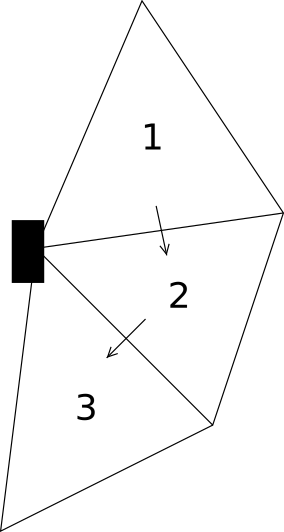
\includegraphics[width=\textwidth]{three_triangles}
    \end{minipage}
  \end{example}
\end{frame}

\begin{frame}{Courant condition \& unstructured}
  Courant condition depends on numerical scheme.
  \begin{example}
    \small
    \begin{minipage}{0.7\textwidth}
    For first order upwind finite volume, the concentration in cell 2 is given
    by
    \begin{equation*}
      c^{n+1}_2 = \left(1-\frac{\Delta t~u_n w}{A_2}\right) c^n_2
        +\frac{\Delta t~u_n w}{A_2} c^n_1
    \end{equation*}

    Rewriting $u_n=\|u\| \hat u\cdot\vec n$, this leads to a CFL condition:
    \begin{equation*}
        \frac{\Delta t~\|u\| \hat u\cdot\vec n~w}{A_2}<1
    \end{equation*}
    In other words $\Delta x=\frac{A_2 \hat u\cdot\vec n}w$.
    \end{minipage}%
    \begin{minipage}{0.3\textwidth}
    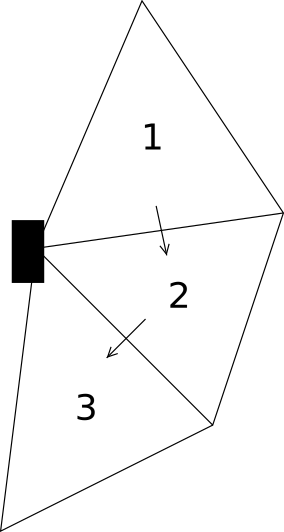
\includegraphics[width=\textwidth]{three_triangles}
  \end{minipage}

\end{example}
\end{frame}

\begin{frame}{Implicit Euler\hspace{10ex}.}
  \begin{textblock}{0.3}(.8,0)
     \includegraphics[width=\textwidth]{backward-euler.png}
  \end{textblock}
  \begin{minipage}{0.7\textwidth}
  The implicit \emph{backward Euler} \\
  time-integration method gives:
  \begin{equation*}
    \mat M\frac{\vT^{n+1}-\vT^n}{\Delta t} 
    + \mat A(\vec u) \vT^{n+1} + \mat D \vT^{n+1} = 0
  \end{equation*}
  or
  \begin{equation*}
    \left[ \mat M + \Delta t\left(\mat A(\vec u) + \mat D\right) \right] \vT^{n+1} = \mat M \vT^n 
  \end{equation*}
  \end {minipage}

  \vspace{1ex}
  This method is \emph{unconditionally} stable, i.e. no time step restriction.

  \vspace{1em}
  However it may introduce excessive damping!
\end{frame}

\begin{frame}{Theta method}
  The theta method is given by:
  \begin{equation*}
    \mat M\frac{\vT^{n+1}-\vT^n}{\Delta t} 
    + \mat A(\vec u) \vT^{n+\theta} + \mat D
    \vT^{n+\theta} = 0
  \end{equation*}
  where
  \begin{equation*}
    T^{n+\theta}=(1-\theta) T^n + \theta T^{n+1}.
  \end{equation*}
  For %
  \begin{tabular}{lll}
    $\theta=0$ & Explicit Euler & conditionally stable \\
    $\theta=1$ & Implicit Euler & uncond. stable, dissipative\hspace{-4em}\;\\
    $\theta=0.5$ & Crank-Nicolson & second order!
  \end{tabular}

  \vspace{1em}
  Unconditionally stable for $\theta>=0.5$. In practice, a value just above
  $0.5$ is often chosen.
\end{frame}

\section{Scalar advection-diffusion}
\begin{frame}{Conservative vs non-conservative}
  \small
  The scalar advection diffusion equation can be solved in two
  forms:
  \begin{align*}
    &\text{Non-conservative form:} &
    \ppt T + \vec u\cdot\grad T - \kappa \nabla^2 T &= 0 \\
    &\text{Conservation form:} &
    \ppt T + \div \left(\vec u T\right) - \kappa \nabla^2 T &= 0.
  \end{align*}

  For smooth fields $T$ in incompressible flow the two should be the same. However, numerically
  $\div\vec u$ is only zero in approximation (depends on pressure
  discretisation). We provide a choice via a
  parameter $\beta$:
  \begin{equation*}
    \ppt T + (1-\beta)\vec u\cdot\grad T + \beta \div \left( \vec u T\right)- \kappa \nabla^2 T = 0.
  \end{equation*}

  \vspace{-0.5em}
  \begin{columns}
    \begin{column}{0.5\textwidth}
      \begin{block}{$\beta=0$, non-conservative}
        Depending on scheme, may be bounded.
      \end{block}
    \end{column}%
    \begin{column}{0.5\textwidth}
      \begin{block}{$\beta=1$, conservative}
        Depending on scheme,
        typically \emph{not} bounded.
      \end{block}
    \end{column}
  \end{columns}
\end{frame}

\begin{frame}{Discretisation for advection-diffusion}
  Three methods:
  \begin{itemize}
    \item Continuous Galerkin
    \item Control Volumes (Finite Volume)
    \item Discontinuous Galerkin
  \end{itemize}
\end{frame}

\begin{frame}{Continuous Galerkin}
  \begin{columns}
  \begin{column}{0.5\textwidth}
  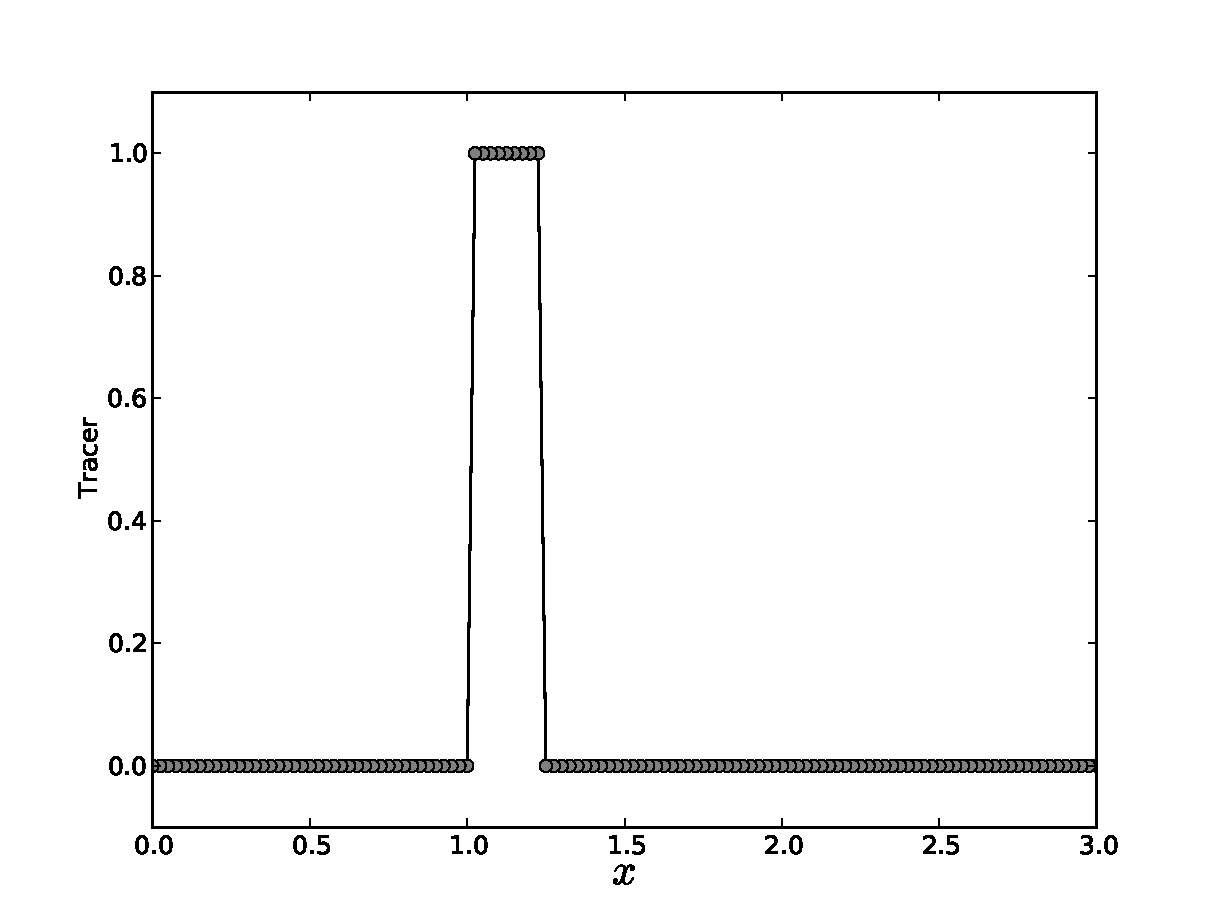
\includegraphics[width=1\textwidth]{tophat0}
  \end{column}
  \begin{column}{0.5\textwidth}
  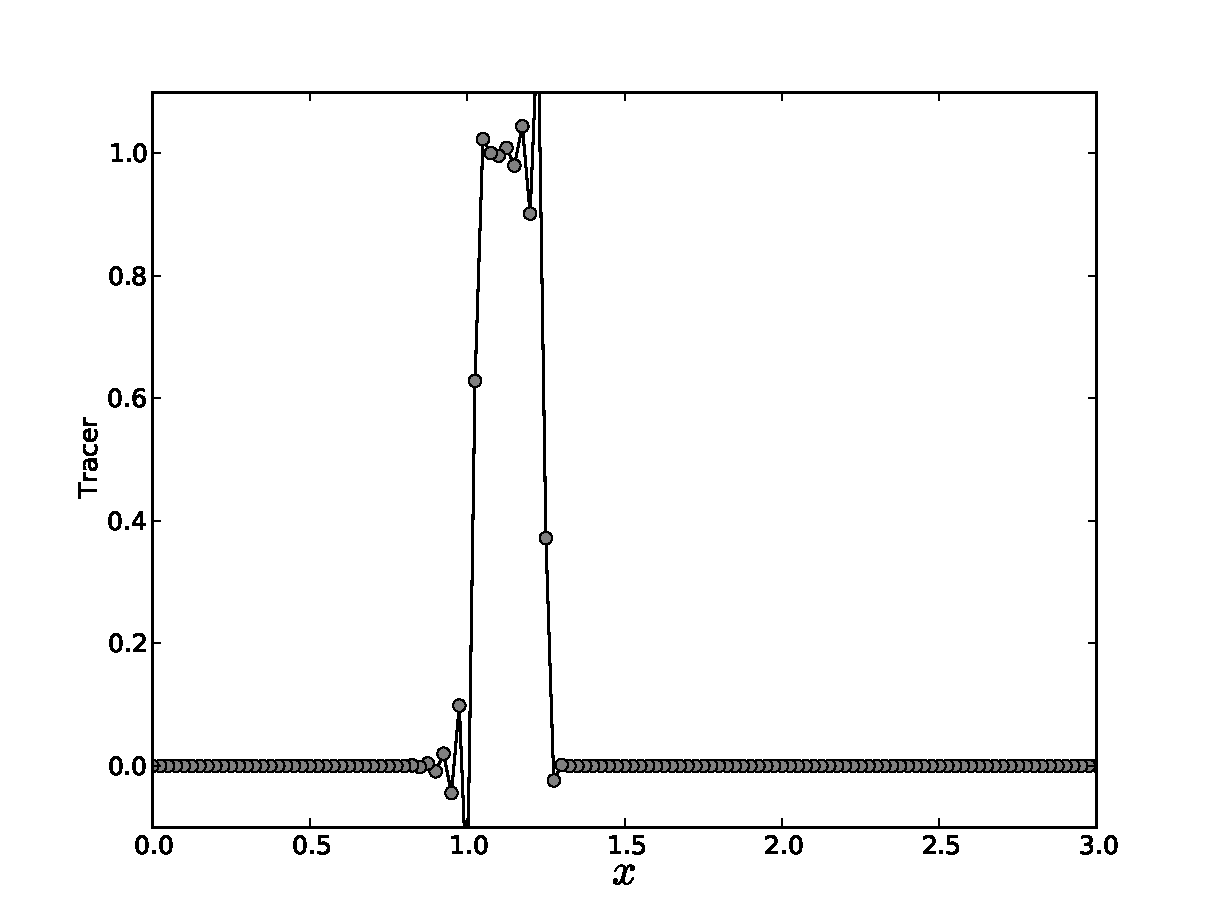
\includegraphics[width=1\textwidth]{tophatcg1}
  \end{column}
  \end{columns}
  Unstabilised Continuous Galerkin is not very good at handling discontinuities
  and large gradients. It is accurate and fairly efficient for smooth fields.

  \begin{columns}
  \begin{column}{0.5\textwidth}
    \begin{block}{Stabilisation methods}
  \begin{itemize}
    \item SU (recommended)
    \item SUPG
  \end{itemize}
\end{block}
  \end{column}%
  \begin{column}{0.49\textwidth}
    {\bf More details see:}\\
    \citet{Donea2003}
  \end{column}
  \end{columns}
\end{frame}

\begin{frame}{Control volumes}
  \begin{columns}
  \begin{column}{0.5\textwidth}%
  Vertex based control volumes

  Face values computed as:
  \begin{itemize}
    \item First order upwind
    \item Finite element (linear interpolation)
  \end{itemize}
  In combination with slope limiter: Sweby
  \end{column}%
  \begin{column}{0.5\textwidth}%
    \hspace{-0.3\textwidth}
  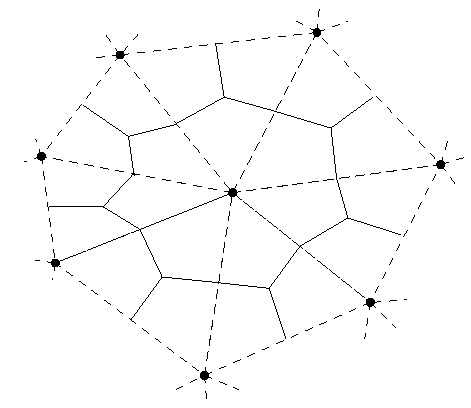
\includegraphics[width=1.2\textwidth]{corner_unstructured_cv_tex}
  \end{column}%
  \end{columns}

  {\bf References:} \\
  \citet{Leveque2002} (general finite volume and slope limiters) \\
  \citet{Wilson2009} (Fluidity specific details, multi-material)
\end{frame}

\begin{frame}{Discontinuous Galerkin}
  \begin{columns}
  \begin{column}{0.5\textwidth}
    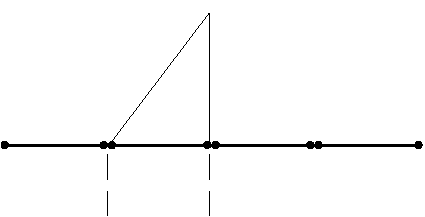
\includegraphics[width=\textwidth,clip,trim=0 30 0
    0]{P1dgshapefunction1d_tex}
  \end{column}
  \begin{column}{0.5\textwidth}
    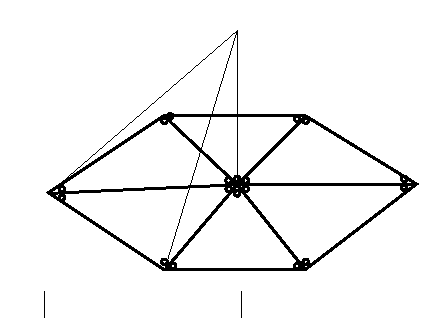
\includegraphics[width=\textwidth,clip,trim=0 20 0
    0]{P1dgshapefunction2d_tex}
  \end{column}
  \end{columns}
  Discontinuous Galerkin methods are much better at handling discontinuities.
  Requires:
  \begin{itemize}
    \item subcycling: advection is divided in small sub-timesteps 
      with CFL number smaller than one.
    \item slope limiting: changes the slope within each element to
      prevent overshoots.
  \end{itemize}
  {\bf Reference:} \cite{Cockburn2001}
\end{frame}

\begin{frame}
  \vspace{-1em}
  \begin{minipage}{0.5\textwidth}
    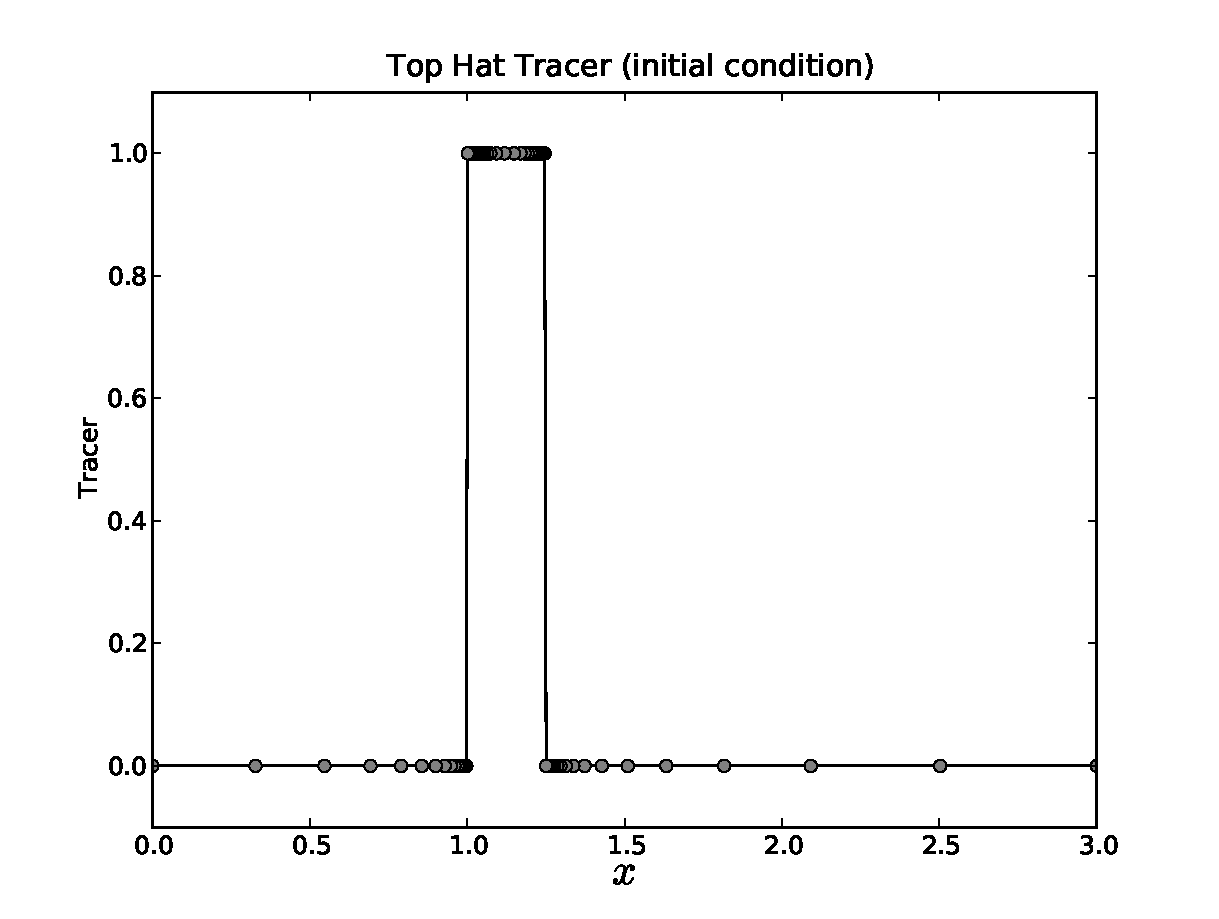
\includegraphics[width=\textwidth]{top_hat_ic}
  \end{minipage}%
  \begin{minipage}{0.5\textwidth}
    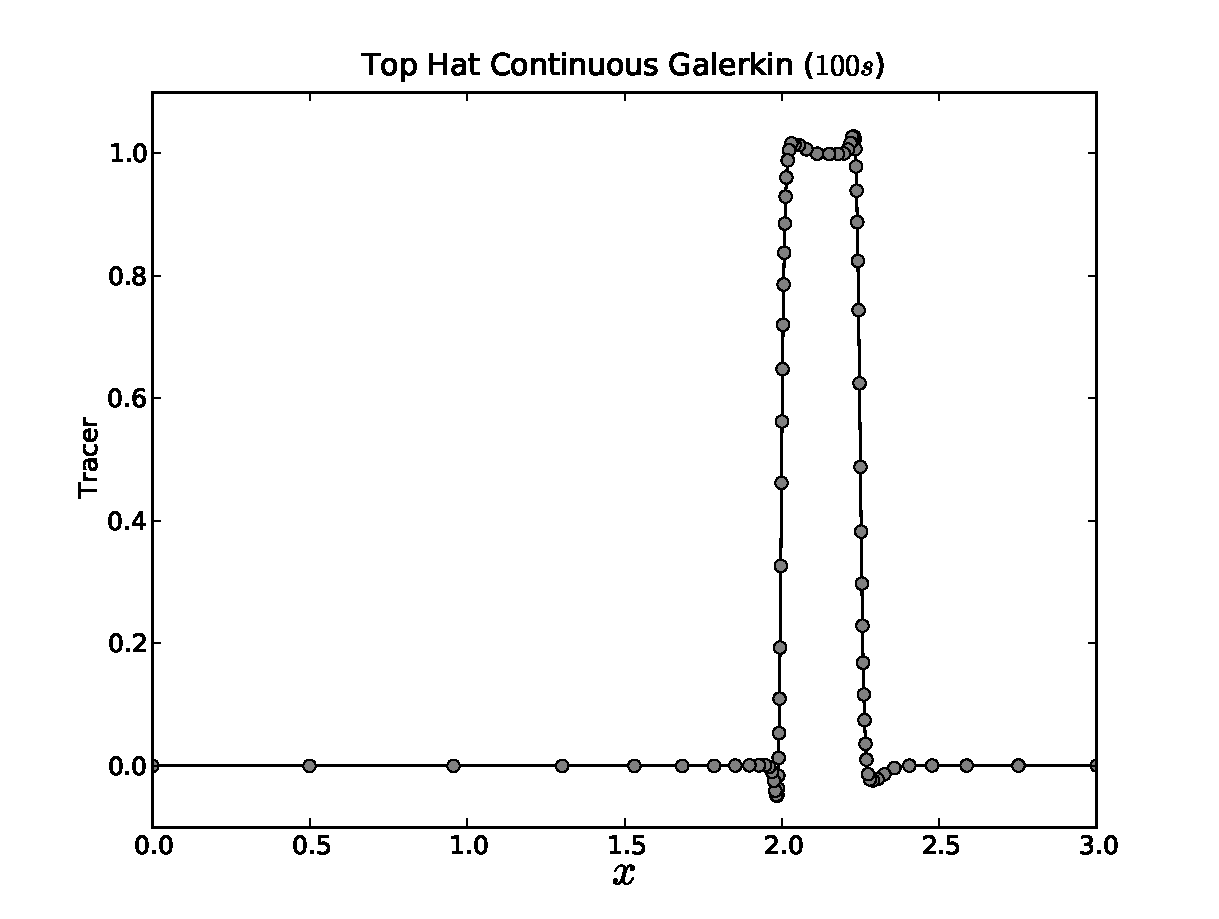
\includegraphics[width=\textwidth]{top_hat_cg}
  \end{minipage}

  \vspace{-1em}
  \begin{minipage}{0.5\textwidth}
    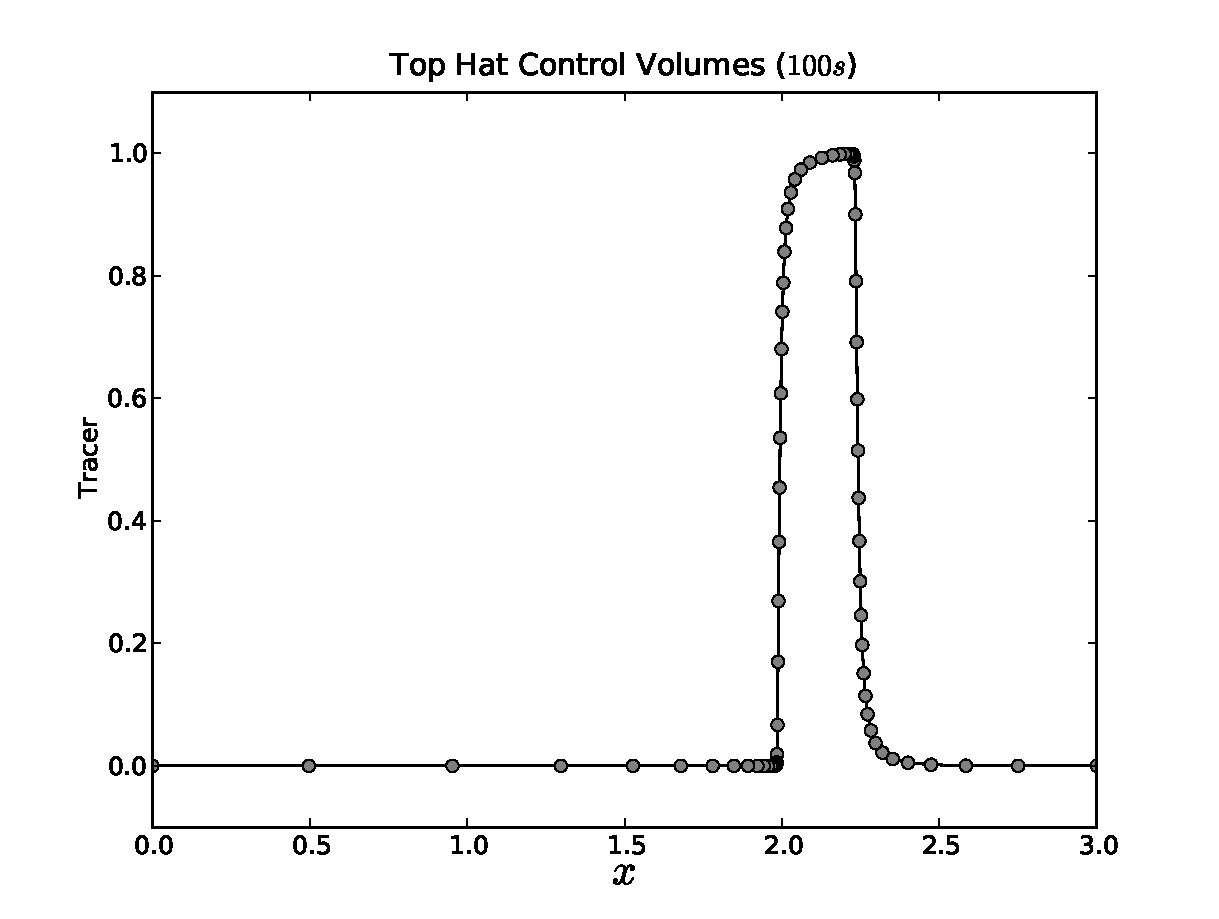
\includegraphics[width=\textwidth]{top_hat_cv}
  \end{minipage}%
  \begin{minipage}{0.5\textwidth}
    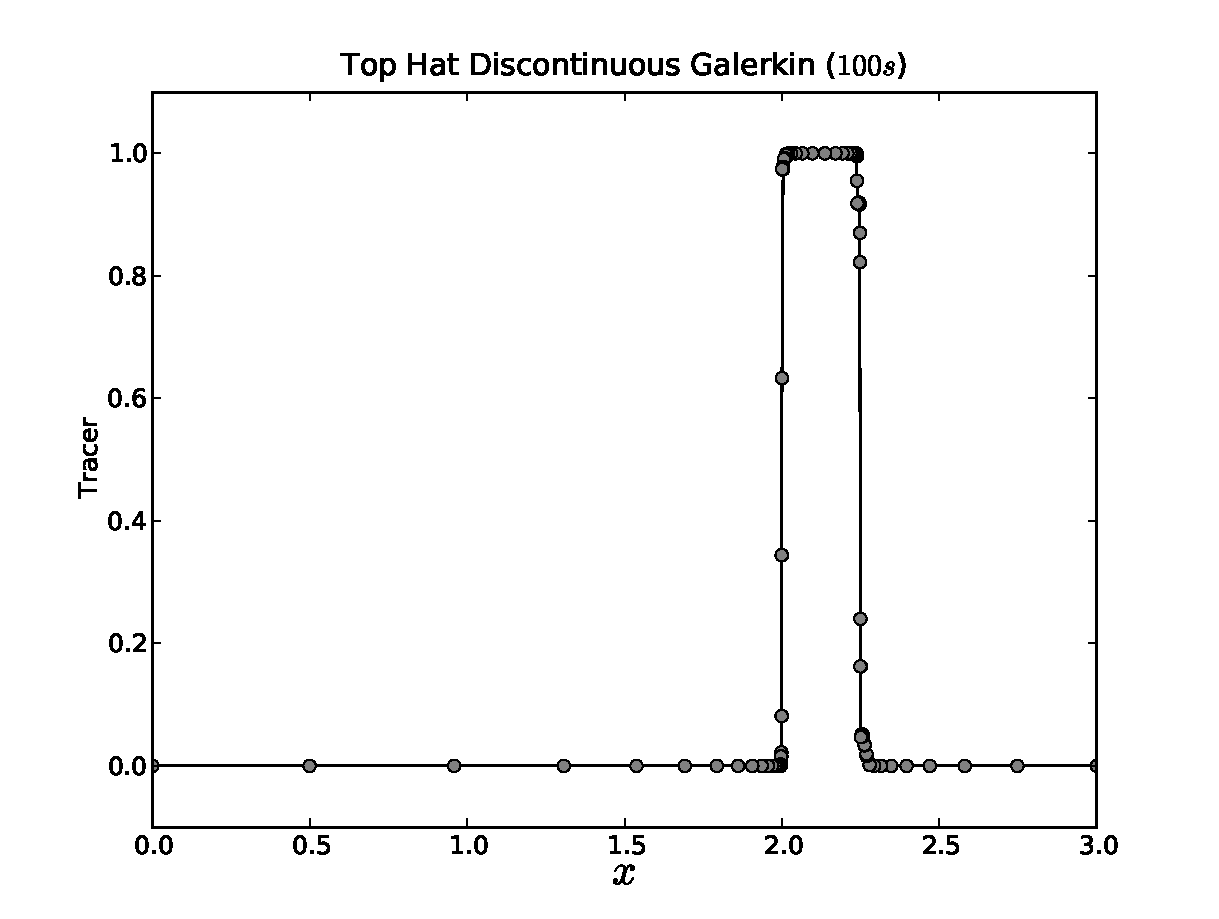
\includegraphics[width=\textwidth]{top_hat_dg}
  \end{minipage}
  \small Top hat example from the Fluidity manual, run with CG+SUPG, 
  and CV+Sweby, and DG+slope limiting.
\end{frame}

\begin{frame}{Diffusion/Viscosity}
  \begin{exampleblock}{Remark:}
    Numerical considerations for the scalar advection diffusion equation are 
    similar to those for the advection and viscosity terms in the momentum equation:
    \begin{align*}
      &\phantom{\rho\big(}\ppt T + \vec u\cdot\grad T - \kappa \nabla^2 T
      = 0. \\
      &\rho\left(\ppt{\vec u} + \vec u\cdot\grad\vec u - \nu \nabla^2 \vec u
      \right)
      + \grad p = -g \rho \hat z 
    \end{align*}
  \end{exampleblock}
\end{frame}

\begin{frame}{Diffusion/Viscosity}
      \vspace{-1em}
  \begin{columns}
    \begin{column}{0.8\textwidth}
      P\'eclet (Reynolds) number, ratio of the rate of advection over the rate of diffusion
      (viscosity):
    \end{column}%
    \begin{column}{0.2\textwidth}
      \vspace{-1em}
  \begin{gather*}
    \mathrm{Pe}=\frac{LU}\kappa\\
    \mathrm{Re}=\frac{LU}\nu
  \end{gather*}
    \end{column}
  \end{columns}
  \begin{columns}
    \begin{column}{0.7\textwidth}
  Typically, the length scale at which diffusion (viscosity) is dominant is much
  smaller than the grid scale:
    \end{column}%
    \begin{column}{0.3\textwidth}
  \begin{gather*}
        \mathrm{Pe}_{\text{grid}}=\frac{\Delta xU}\kappa\ \gg 1\\
        \mathrm{Re}_{\text{grid}}=\frac{\Delta xU}\nu \gg 1
  \end{gather*}
    \end{column}
  \end{columns}

  \begin{block}{Sub-grid/turbulence models}
    \begin{itemize}
      \item RANS models: k-$\epsilon$ model
      \item Large Eddy simulation (LES)
      \item Vertical parameterisations for oceans: GLS model.
    \end{itemize}
  \end{block}
  {\bf References:} LES and k-$\epsilon$: \citet{Pope2000,Wilcox1998},
  GLS: \citet{Hill2012,Umlauf2005}
\end{frame}

\section{Incompressible Navier Stokes}
\begin{frame}{Incompressible NS equations}
  Incompressible Navier Stokes equations:
  \begin{gather*}
    \rho\ppt{\vec u} + \rho\vec u\cdot\grad\vec u - \mu \nabla^2 \vec u 
      + \grad p = -g \rho \hat z \\
    \div \vec u =0
  \end{gather*}
  with density $\rho$, velocity $\vec u$, dynamic viscosity $\mu$, 
  pressure $p$, gravitational acceleration $g$, and $\hat z$ the upwards unit
  vector. Density from equation of state:
  \begin{equation*}
    \rho = \rho_0 \left( 1 - \alpha T + \gamma S\right),
  \end{equation*}
  where $\rho_0$ is the reference density, $T$ and $S$ are temperature and
  salinity, and $\alpha$ and $\gamma$ are the thermal expansion and haline
  contraction coefficients.
\end{frame}

\begin{frame}{Incompressible NS equations}
  Incompressible Navier Stokes equations in the \emph{Boussinesq} approximation:
  ($|\rho-\rho_0|\ll \rho_0$)
  \begin{gather*}
    \rho_0\ppt{\vec u} + \rho_0\vec u\cdot\grad\vec u - \mu \nabla^2 \vec u 
      + \grad p = -g \rho \hat z \\
    \div \vec u =0
  \end{gather*}
  with density $\rho$, velocity $\vec u$, dynamic viscosity $\mu$, 
  pressure $p$, gravitational acceleration $g$, and $\hat z$ the upwards unit
  vector. Density from equation of state:
  \begin{equation*}
    \rho = \rho_0 \left( 1 - \alpha T + \gamma S\right),
  \end{equation*}
  where $\rho_0$ is the reference density, $T$ and $S$ are temperature and
  salinity, and $\alpha$ and $\gamma$ are the thermal expansion and haline
  contraction coefficients.
\end{frame}

\begin{frame}{Incompressible NS equations}
  Incompressible Navier Stokes equations in the \emph{Boussinesq} approximation:
  ($|\rho-\rho_0|\ll \rho_0$)
  \begin{gather*}
    \ppt{\vec u} + \vec u\cdot\grad\vec u - \nu \nabla^2 \vec u 
    + \grad P = -g \frac\rho{\rho_0} \hat z \\
    \div \vec u =0
  \end{gather*}
  with density $\rho$, velocity $\vec u$, kinematic viscosity $\nu=\mu/\rho_0$, 
  kinematic pressure $P=p/\rho_0$, gravitational acceleration $g$, and $\hat z$ the upwards unit
  vector. Density from equation of state:
  \begin{equation*}
    \rho = \rho_0 \left( 1 - \alpha T + \gamma S\right),
  \end{equation*}
  where $\rho_0$ is the reference density, $T$ and $S$ are temperature and
  salinity, and $\alpha$ and $\gamma$ are the thermal expansion and haline
  contraction coefficients.
\end{frame}

\begin{frame}{Hydrostatic pressure}
  Large part of pressure is hydrostatic, i.e.
  \begin{equation*}
    \pp{p_h}z = -\rho g,\quad p_h=0\text{ at }z=0 \implies
    p_h=\int_{z'=z}^{z'=0} \rho g ~dz'
  \end{equation*}
  In other words, $p_h$ is proportional to the weight of the water column
  above each point in the fluid. If we only look at the weight of the reference
  fluid, then
  \begin{equation*}
    p_{h,0}=-\rho_0 gz \text{ and } \nabla p_{h,0}=-\rho_0 g \hat z
  \end{equation*}

\end{frame}

\begin{frame}{Hydrostatic pressure}
  Large part of pressure is hydrostatic, i.e.
  \begin{equation*}
    \pp{p_h}z = -\rho g,\quad p_h=0\text{ at }z=0 \implies
    p_h=\int_{z'=z}^{z'=0} \rho g ~dz'
  \end{equation*}
  In other words, $p_h$ is proportional to the weight of the water column
  above each point in the fluid. If we only look at the weight of the reference
  fluid, then
  \begin{equation*}
    p_{h,0}=-\rho_0 gz \text{ and } \nabla p_{h,0}=-\rho_0 g \hat z
  \end{equation*}
\end{frame}

\begin{frame}{Subtract hydrostatic part}
  Pressure is split according to
  \begin{equation*}
    P = P_{h,0} + P'
  \end{equation*}
  where the reference hydrostatic pressure is given by:
  \begin{equation*}
    P_{h,0}=-gz \text{ so that } \nabla P_{h,0}=-g \hat z
  \end{equation*}
  Substitution in the momentum equation:
  \begin{equation*}
    \ppt{\vec u} + \vec u\cdot\grad\vec u - \nu \nabla^2 \vec u 
    + \grad P_{h,0} + \grad P' =
    -\frac{g}{\rho_0}\left(\rho_0+\Delta\rho\right)\hat z
  \end{equation*}
\end{frame}

\definecolor{light-gray}{gray}{0.7}
\newcommand\grayed[1]{{\color{red}\cancel{\color{light-gray} #1}}}
\begin{frame}{Subtract hydrostatic part}
  Pressure is split according to
  \begin{equation*}
    P = P_{h,0} + P'
  \end{equation*}
  where the reference hydrostatic pressure is given by:
  \begin{equation*}
    P_{h,0}=-gz \text{ so that } \nabla P_{h,0}=-g \hat z
  \end{equation*}
  Substitution in the momentum equation:
  \begin{equation*}
    \ppt{\vec u} + \vec u\cdot\grad\vec u - \nu \nabla^2 \vec u 
    \grayed{+ \grad P_{h,0}} + \grad P' =
    -\frac{g}{\rho_0}\left(\grayed{\rho_0+}\Delta\rho\right)\hat z
  \end{equation*}
\end{frame}

\begin{frame}{Free surface and Pressure}
  \begin{minipage}{0.5\textwidth}
    If a free surface is included, with elevation $\eta$, the
    part of the hydrostatic pressure between $z=0$ and $z=\eta$ is \emph{not}
    subtracted.
  \end{minipage}%
  \hspace{0.05\textwidth}%
  \begin{minipage}{0.45\textwidth}
    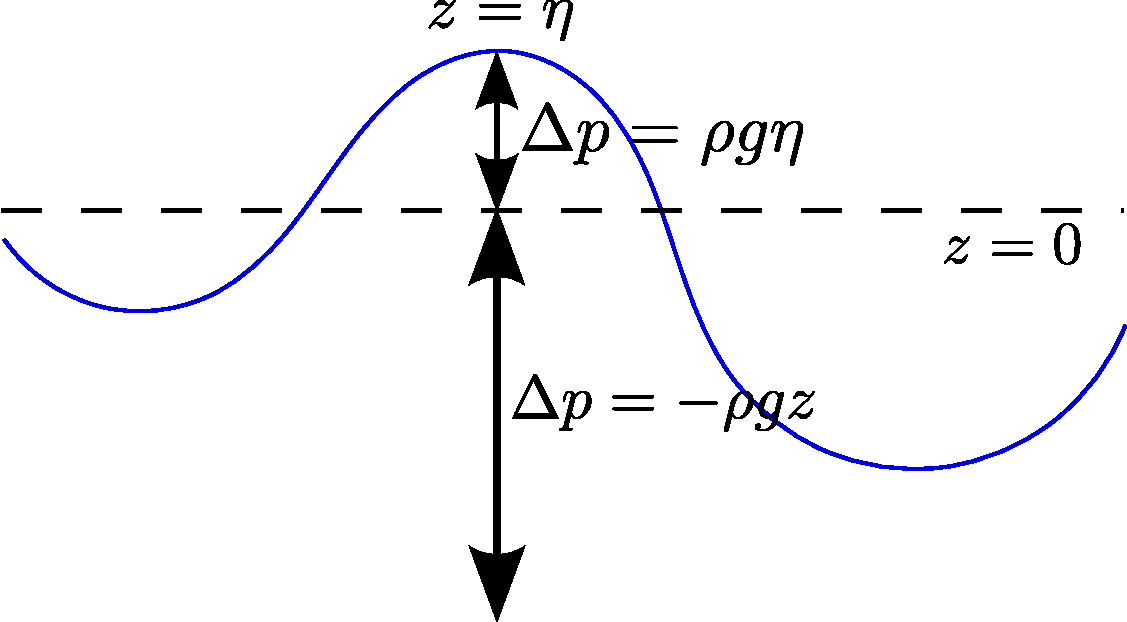
\includegraphics[width=\textwidth]{fs1}
  \end{minipage}
  
  \vspace{1em}
  In other words, the barotropic part of pressure $\rho_0g\eta$ is
  included in the pressure solved for in Fluidity.

  \vspace{1em}
  This means that P' is nonzero at the free-surface, because at $z=\eta$:
  \begin{equation*}
    P' = P-P_{h,0} = 0 + gz |_{z=\eta} = g\eta
  \end{equation*}
\end{frame}

\begin{frame}{Discretisation of NS}
  Boussinesq equations with hydrostatic subtracted:
  \begin{gather*}
    \ppt{\vec u} + \vec u\cdot\grad\vec u - \nu \nabla^2 \vec u 
    + \grad P' = -g \frac{\Delta\rho}{\rho_0} \hat z \\
    \div \vec u =0
  \end{gather*}
  Discretised in time and space:
  \begin{gather*}
    \mat M\frac{\vu^{n+1}-\vu^n}{\Delta t} + \mat A(\vec u)\vu^{n+\theta}
    + \mat K \vu^{n+\theta}
    + \mat C\vp^{n+\tfrac 12} = \vf(\Delta\rho) \\
    -\mat C^T \vu^{n+1} = 0
  \end{gather*}
  \vspace{-1em}
  \begin{exampleblock}{}
    with matrices:
    \begin{tabular}{ll}
      $\mat M$ & mass matrix \\
      $\mat A(\vu)$ & advection matrix \\
      $\mat K$ & viscosity matrix \\
      $\mat C$ & gradient matrix \\
      $-\mat C^T$ & divergence matrix \\
    \end{tabular}
  \end{exampleblock}
\end{frame}
\begin{frame}{Pressure correction approach}
  \vspace{-1em}
  \begin{gather*}
    \ppt{\vec u} + \vec u\cdot\grad\vec u - \nu \nabla^2 \vec u 
    + \grad P' = -g \frac{\Delta\rho}{\rho_0} \hat z \\
    \div \vec u =0
  \end{gather*}
  Solved in three steps:
  \begin{enumerate}
    \item Solve a preliminary $\vu^{\ast}$ (not divergence free):
      \begin{equation*}
        \mat M\frac{\vu^\ast-\vu^n}{\Delta t} + \mat A(\vec u)\vu^{n+\theta} +
        \mat K \vu^{n+\theta}
        + \mat C\vp^{n-\tfrac 12} = \vf
      \end{equation*}
    \item Solve pressure correction $\delta\vp$:
      \begin{equation*}
        \mat C^T \mat M^{-1} \mat C ~ \delta\vp = -\mat C^T \vu^*
      \end{equation*}
    \item Correct velocity, and update pressure:
      \begin{equation*}
        \mat M\frac{\vu^{n+1}-\vu^\ast}{\Delta t} + \mat C\delta\vp =0,\quad
        \vp^{n+\tfrac 12} = \vp^{n-\tfrac 12} + \delta\vp
      \end{equation*}
  \end{enumerate}
  {\small{\bf More details:}\citet{Gresho1998}}
\end{frame}

\begin{frame}{Choice of velocity, pressure pair}
  \vspace{-1em}
  \begin{columns}
    \begin{column}{0.5\textwidth}
      \begin{exampleblock}{\poo}
        Advantages:
        \begin{enumerate}
          \item Simple
        \end{enumerate}
        Disadvantages:
        \begin{enumerate}
          \item Unstable (LBB criterion), requires additional stabilisation
          \item Mass lumping required
        \end{enumerate}
      \end{exampleblock}
    \end{column}
    \begin{column}{0.5\textwidth}
      \begin{exampleblock}{\podgpt}
        Advantages:
        \begin{enumerate}
          \item Higher order
          \item Geostrophic balance
          \item Stable
          \item No mass lumping
        \end{enumerate}
        Disadvantages:
        \begin{enumerate}
          \item More DOFs
        \end{enumerate}
      \end{exampleblock}
    \end{column}
  \end{columns}

  \vspace{-0.5em}
  \begin{columns}
    \begin{column}{0.25\textwidth}
      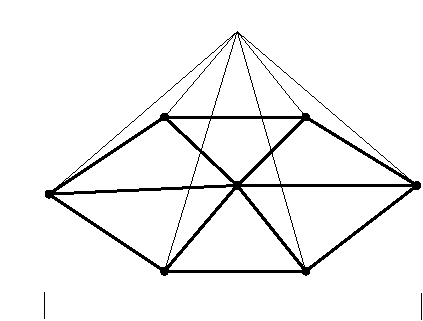
\includegraphics[width=\textwidth,clip,trim=0 20 0 0]{P1cgshapefunction2d_tex}

      \bf\centering\tiny Velocity
    \end{column}
    \begin{column}{0.25\textwidth}
      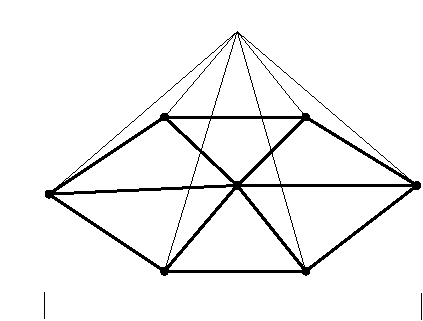
\includegraphics[width=\textwidth,clip,trim=0 20 0 0]{P1cgshapefunction2d_tex}

      \bf\centering\tiny Pressure
    \end{column}
    \begin{column}{0.25\textwidth}
      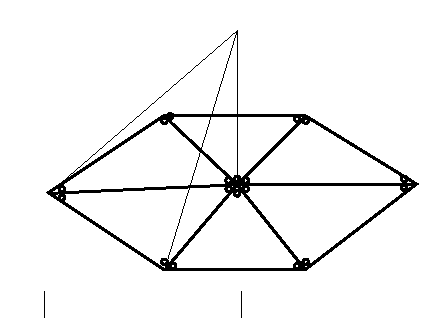
\includegraphics[width=\textwidth,clip,trim=0 20 0 0]{P1dgshapefunction2d_tex}

      \bf\centering\tiny Velocity
    \end{column}
    \begin{column}{0.25\textwidth}
      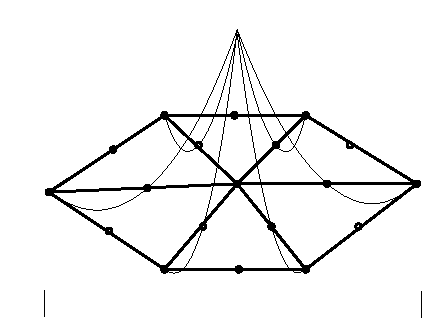
\includegraphics[width=\textwidth,clip,trim=0 20 0 0]{P2cgshapefunction2d_tex}

      \bf\centering\tiny Pressure
    \end{column}
  \end{columns}
  \vspace{0.5em}

  \footnotesize
  {\bf References:} \citet{Gresho1998} (element pairs, LBB stability),
  \citet{Cotter2009} (\podgpt),
  \citet{Pain2005} (\poo\ stabilisation)
\end{frame}

\begin{frame}{Geostrophic balance}
  \small
  In larger scale ocean simulations, the flow is dominated by a
  \emph{geostrophic balance} between the pressure gradient and
  Coriolis term in the horizontal, and \emph{hydrostatic balance}
  in the vertical: 
  \begin{equation*}
    {\color{gray}
    \ppt{\vec u} + \vec u\cdot\grad\vec u - \nu \nabla^2 \vec u + }
      2\vec \Omega \times \vec u
      + \grad P' = -g \frac{\Delta \rho}{\rho_0} \hat z,
    \end{equation*}
    here $\vec\Omega$ is the angular velocity vector of the Earth's
    rotation.

    \vspace{1em}
    The gradient of a P1 pressure is P0 (piece-wise constant); Therefore,
    no exact balance between a P1 Coriolis term (or P1 buoyancy). With
    \emph{\poo} we
    solve for a separate \emph{geostrophic pressure} that is piecewise
    quadratic (P2, still no exact balance). With \emph{\podgpt} an exact balance
    is possible without a separate
    geostrophic pressure solve.
\end{frame}

\section{Time loop}
\newcommand\eqbox[2]{\small #1:\\{\scriptsize #2}}
% Frame starts a new slide
\begin{frame}[fragile]
  \only<1>{\frametitle{Time loop}}
  \pgfdeclarelayer{nsbackground}
  \pgfdeclarelayer{itinoibackground}
  \pgfsetlayers{itinoibackground,nsbackground,main}
  % fonts have been chosen above in eqbox def - this only affects spacing
  \tiny
  % Define block styles
  \tikzstyle{line} = [draw]
  \tikzstyle{cloud} = [draw, rectangle, rounded corners,
  fill=white, minimum height=2em,text width=0.6\textwidth, text centered]
  \tikzstyle{tscloud} = [cloud,text width=0.45\textwidth]
  \tikzstyle{eoscloud} = [cloud,text width=0.45\textwidth]

  \vspace{-2em}
  \begin{tikzpicture}[node distance=1.0em]
    % define nodes and put text
    \node [tscloud] (temperature) {
      \eqbox{Temperature}
      {$\frac{T^{n+1}-T^n}{\Delta t} + \vec u\cdot\grad T^{n+\theta} 
       - \kappa_T \nabla^2 T^{n+\theta} = 0$}};
    \node [tscloud, right=of temperature] (salinity) {
      \eqbox{Salinity}
      {$\frac{S^{n+1}-S^n}{\Delta t} + \vec u\cdot\grad S^{n+\theta}
       - \kappa_S \nabla^2 S^{n+\theta} = 0$}};
    \node [node distance=auto, fit=(temperature) (salinity)] (tempsal) {};
    \node [cloud, fill=blue!20, below=of tempsal,text width=0.3\textwidth]
    (eos) {
      \eqbox{Equation of State}
      {$\rho=\rho_0(1-\alpha T+\gamma S)$}};
    \node [node distance=2em,cloud, below=of eos] (momentum) {
      \eqbox{Momentum}
      {$\frac{\vec u^*-\vec u^n}{\Delta t} + \vec u\cdot\nabla\vec u^{n+\theta} 
       - \nu \nabla^2 \vec u^{n+\theta} + \grad P'^{n-\tfrac 12} =
       -g\frac{\rho}{\rho_0}\hat z$}};
    \node [cloud, below=of momentum] (pressure) {
      \eqbox{Pressure}
      {$\nabla^2 \delta P' = - \div\vec u^*$}};
    \node [cloud, below=of pressure] (velcor) {
      \eqbox{Velocity correction}
      {$\frac{\vec u^{n+1}-\vec u^*}{\Delta t} + \grad \delta P' = 0$}};
    % draw edges
    \begin{pgfonlayer}{nsbackground}
      \node [cloud,fill=blue!40, fit=(momentum) (pressure) (velcor)] (ns) {};
    \end{pgfonlayer}
    % some auxiliary points
    \node [above=of tempsal] (above eos) {};
    \node (a) at (eos.west -| -2.6,0) {};
    \node (b) at (a |- temperature.north) {};
    \node (c) at (-2,0.8) {};
    \node (d) at (-0.5,0.8) {};
    \node (e) at (5,0.8) {};
    \draw [->,thick] (eos) -- (ns);
    \draw [->,thick] (temperature) -- (eos);
    \draw [->,thick] (salinity) -- (eos);
    \pause
    \draw [->,thick] (ns.west) to[out=-180,in=-90] 
      node [fill=black!10,align=center] {
        $i=1,\dots N$ or \\ 
        until $\max |\Delta f|<\epsilon$
      } (a) 
      to [out=90,in=-90] (b) to
    [out=90,in=180] (c) to [out=0,in=180] (d) to [out=0,in=90] (temperature.north);
    \draw [->,thick] (c) to [out=0,in=180] (e) to [out=0,in=90] (salinity.north);
    \begin{pgfonlayer}{itinoibackground}
    \node [cloud, drop shadow, fill=blue!80, fit=(ns) (a) (c) (salinity)] (itinoi) {};
    \end{pgfonlayer}

    \pause
    \node [cloud,drop shadow,fill=green,below=of itinoi] (diagnostic) {\large Diagnostic fields};
    \node [cloud,drop shadow,fill=red,above=of itinoi] (prescribed) {\large
    Prescribed fields};

    \draw [->,thick] (prescribed) to (itinoi);
    \draw [->,thick] (itinoi) to (diagnostic);
  \end{tikzpicture}

  \only<2>{
  \vspace{-3em}
  {\normalsize\bf Non-linear (Picard) iteration} \\
  \small Specified number of iterations $N$ (often $N=2$) or until changes in
  prognostic field values are small enough. Advective velocity is updated
  according to a seperate $\theta$, the \emph{relaxation} parameter.}
\end{frame}

\begin{frame}{Baroclinic instability}
  Due to a lack of coupling between momentum and temperature equation, there
  is a numerical instability associated with the buoyancy frequency
  \begin{equation*}
    N^2 = -\frac g{\rho_0}\pp\rho{z}.
  \end{equation*}
  This leads to a time step restriction of
  \begin{equation*}
    N\Delta t<1.
  \end{equation*}
  Fluidity provides an option, called
  {\bf\lstinline{implicit_buoyancy}}, to overcome
  this restriction.
\end{frame}

\section{Boundary conditions}
\begin{frame}{Strong vs. weak boundary conditions}
  \begin{itemize}
    \item \emph{Strong} boundary conditions are imposed exactly in each node of the mesh
    \item \emph{Weak} boundary conditions are imposed in a weak integral sense
      that occur naturally in the finite element discretisation
  \end{itemize}
  \begin{example}
  Weak FEM discretisation of advection equation:
  \begin{equation*}
    \int_\Omega \psi\ppt T + \int_\Omega \psi \vec u\cdot\grad T =0,\quad
    \text{for all }\psi\in V_{\text{test}}
  \end{equation*}
  Integrate by parts\only<2>{, substitute boundary condition $T=T_D$}:
  \only<1>{
  \begin{equation*}
    \int_\Omega \psi\ppt T - \int_\Omega \grad\psi \cdot \vec uT 
    +\int_\Gamma \psi\vec n\cdot\vec u T =0,\quad
    \text{for all }\psi\in V_{\text{test}}
  \end{equation*}}%
  \only<2>{
  \begin{equation*}
    \int_\Omega \psi\ppt T - \int_\Omega \grad\psi \cdot \vec uT 
    +\int_\Gamma \psi\vec n\cdot\vec u T_D =0,\quad
    \text{for all }\psi\in V_{\text{test}}
  \end{equation*}}%
\end{example}
\end{frame}

\begin{frame}{Strong vs. weak boundary conditions}
  \begin{itemize}
    \item \emph{Strong} boundary conditions are imposed exactly in each node of the mesh
    \item \emph{Weak} boundary conditions are imposed in a weak integral sense
      that occur naturally in the finite element discretisation
  \end{itemize}
  Weak are generally better behaved. Although the boundary condition is not
  satisfied exactly, integrated quantities such as fluxes through the
  boundaries are exact. Neumann boundary conditions are always weakly imposed.

  Strong boundary conditions should only be used in special cases.
\end{frame}

\begin{frame}{BCs for scalar advection-diffusion}
  \begin{itemize}
    \item {\bf Dirichlet}: weakly or strongly implied. Required at inflow
      boundary. Unstable for outflow boundary. At a closed boundary ($\vec
      u\cdot\vec n=0$) only works
      in combination with diffusion.
    \item {\bf Neumann}: typically only applied at a closed boundary. The value
      $g$ that is provided specifies the diffusive flux:
      \begin{equation*}
        \kappa \vec n\cdot\grad T = g
      \end{equation*}
    \item {\bf Robin}: Only works with CV and CG. Specify values $C_0$ and $C_1$ such that:
      \begin{equation*}
        C_1 T + \kappa \vec n\cdot\grad T = C_0
      \end{equation*}
  \end{itemize}
\end{frame}

\begin{frame}{BCs for incompressible Navier Stokes}
  Dirichlet bcs are applied to velocity components individually. Choice between:
  \begin{itemize}
    \item \emph{Cartesian aligned}. Specify bcs for $u$,$v$ and $w$ components (in
      $x, y$ and $z$ directions). Works well in Cartesian, box-like domains or
      if all components are specified.
    \item \emph{Surface aligned} (also known as \emph{rotated boundary
      conditions}). Specify bcs in normal and tangential directions
      respectively. Requires computation of normal vectors on the nodes. Can usually be
      avoided.
  \end{itemize}
\end{frame}

\begin{frame}{BCs for incompressible Navier Stokes}

  {\bf Closed boundaries}
  \begin{itemize}
    \item {\bf No slip:} Apply Dirichlet boundary conditions in all directions
      (weakly or strongly), setting all components to zero.
    \item {\bf Free slip:} Recommended: apply the so called \lstinline{no_normal_flow}
      boundary condition to weakly impose the no normal flow condition, g.
      This condition can be imposed strongly, but for non-Cartesian aligned
      domains this requires rotated boundary conditions.
    \item {\bf Bottom or wind drag:} Same as free slip but additionally
      specifying a bottom/wind drag:
      \begin{align*}
        \tau_{\text{bottom}} &= C_D |u|\vec u, \\
        \tau_{\text{wind}} &= C_w \left\|\vec u_{\text wind}-\vec u\right\|
        \left(\vec u_{\text wind}-\vec u\right)
      \end{align*}
  \end{itemize}
\end{frame}

\begin{frame}{BCs for incompressible Navier Stokes}

  Considerations for \emph{open boundaries}:
  \begin{itemize}
    \item For incompressible flows, the inflow has to be the same as the outflow. 
    \item Ideally, only the inflow should be specified.
    \item The influence of the inflow boundary condition is immediately felt throughout the domain.
    \item The outflow condition is
  a free stress condition, which means that a zero pressure is assumed on the
  outside of the domain.
  \end{itemize}
\end{frame}

\begin{frame}{BCs for incompressible Navier Stokes}
  Lateral open boundary conditions are often better behaved in combination
  with a \emph{free surface} condition at the top of the domain. In that case:
  \begin{itemize}
    \item Inflow does not travel immediately across the domain (finite wave speed)
      and  storage of water is possible.
    \item Can specify a velocity boundary condition in both directions (in-
      and outflow), e.g. periodic tidal forcing. Better avoided in
      areas with strong non-linear effects.
    \item Free surface boundary condition is specified through pressure boundary
      condition: $p=g\eta$. Assumes no non-hydrostatic effects and geostrophic pressure 
      should be subtracted.
    \item Velocity boundary conditions on  all open sides easily leads to
      a drift in the total volume.
  \end{itemize}
  
\end{frame}

\begin{frame}{Periodic bcs}
  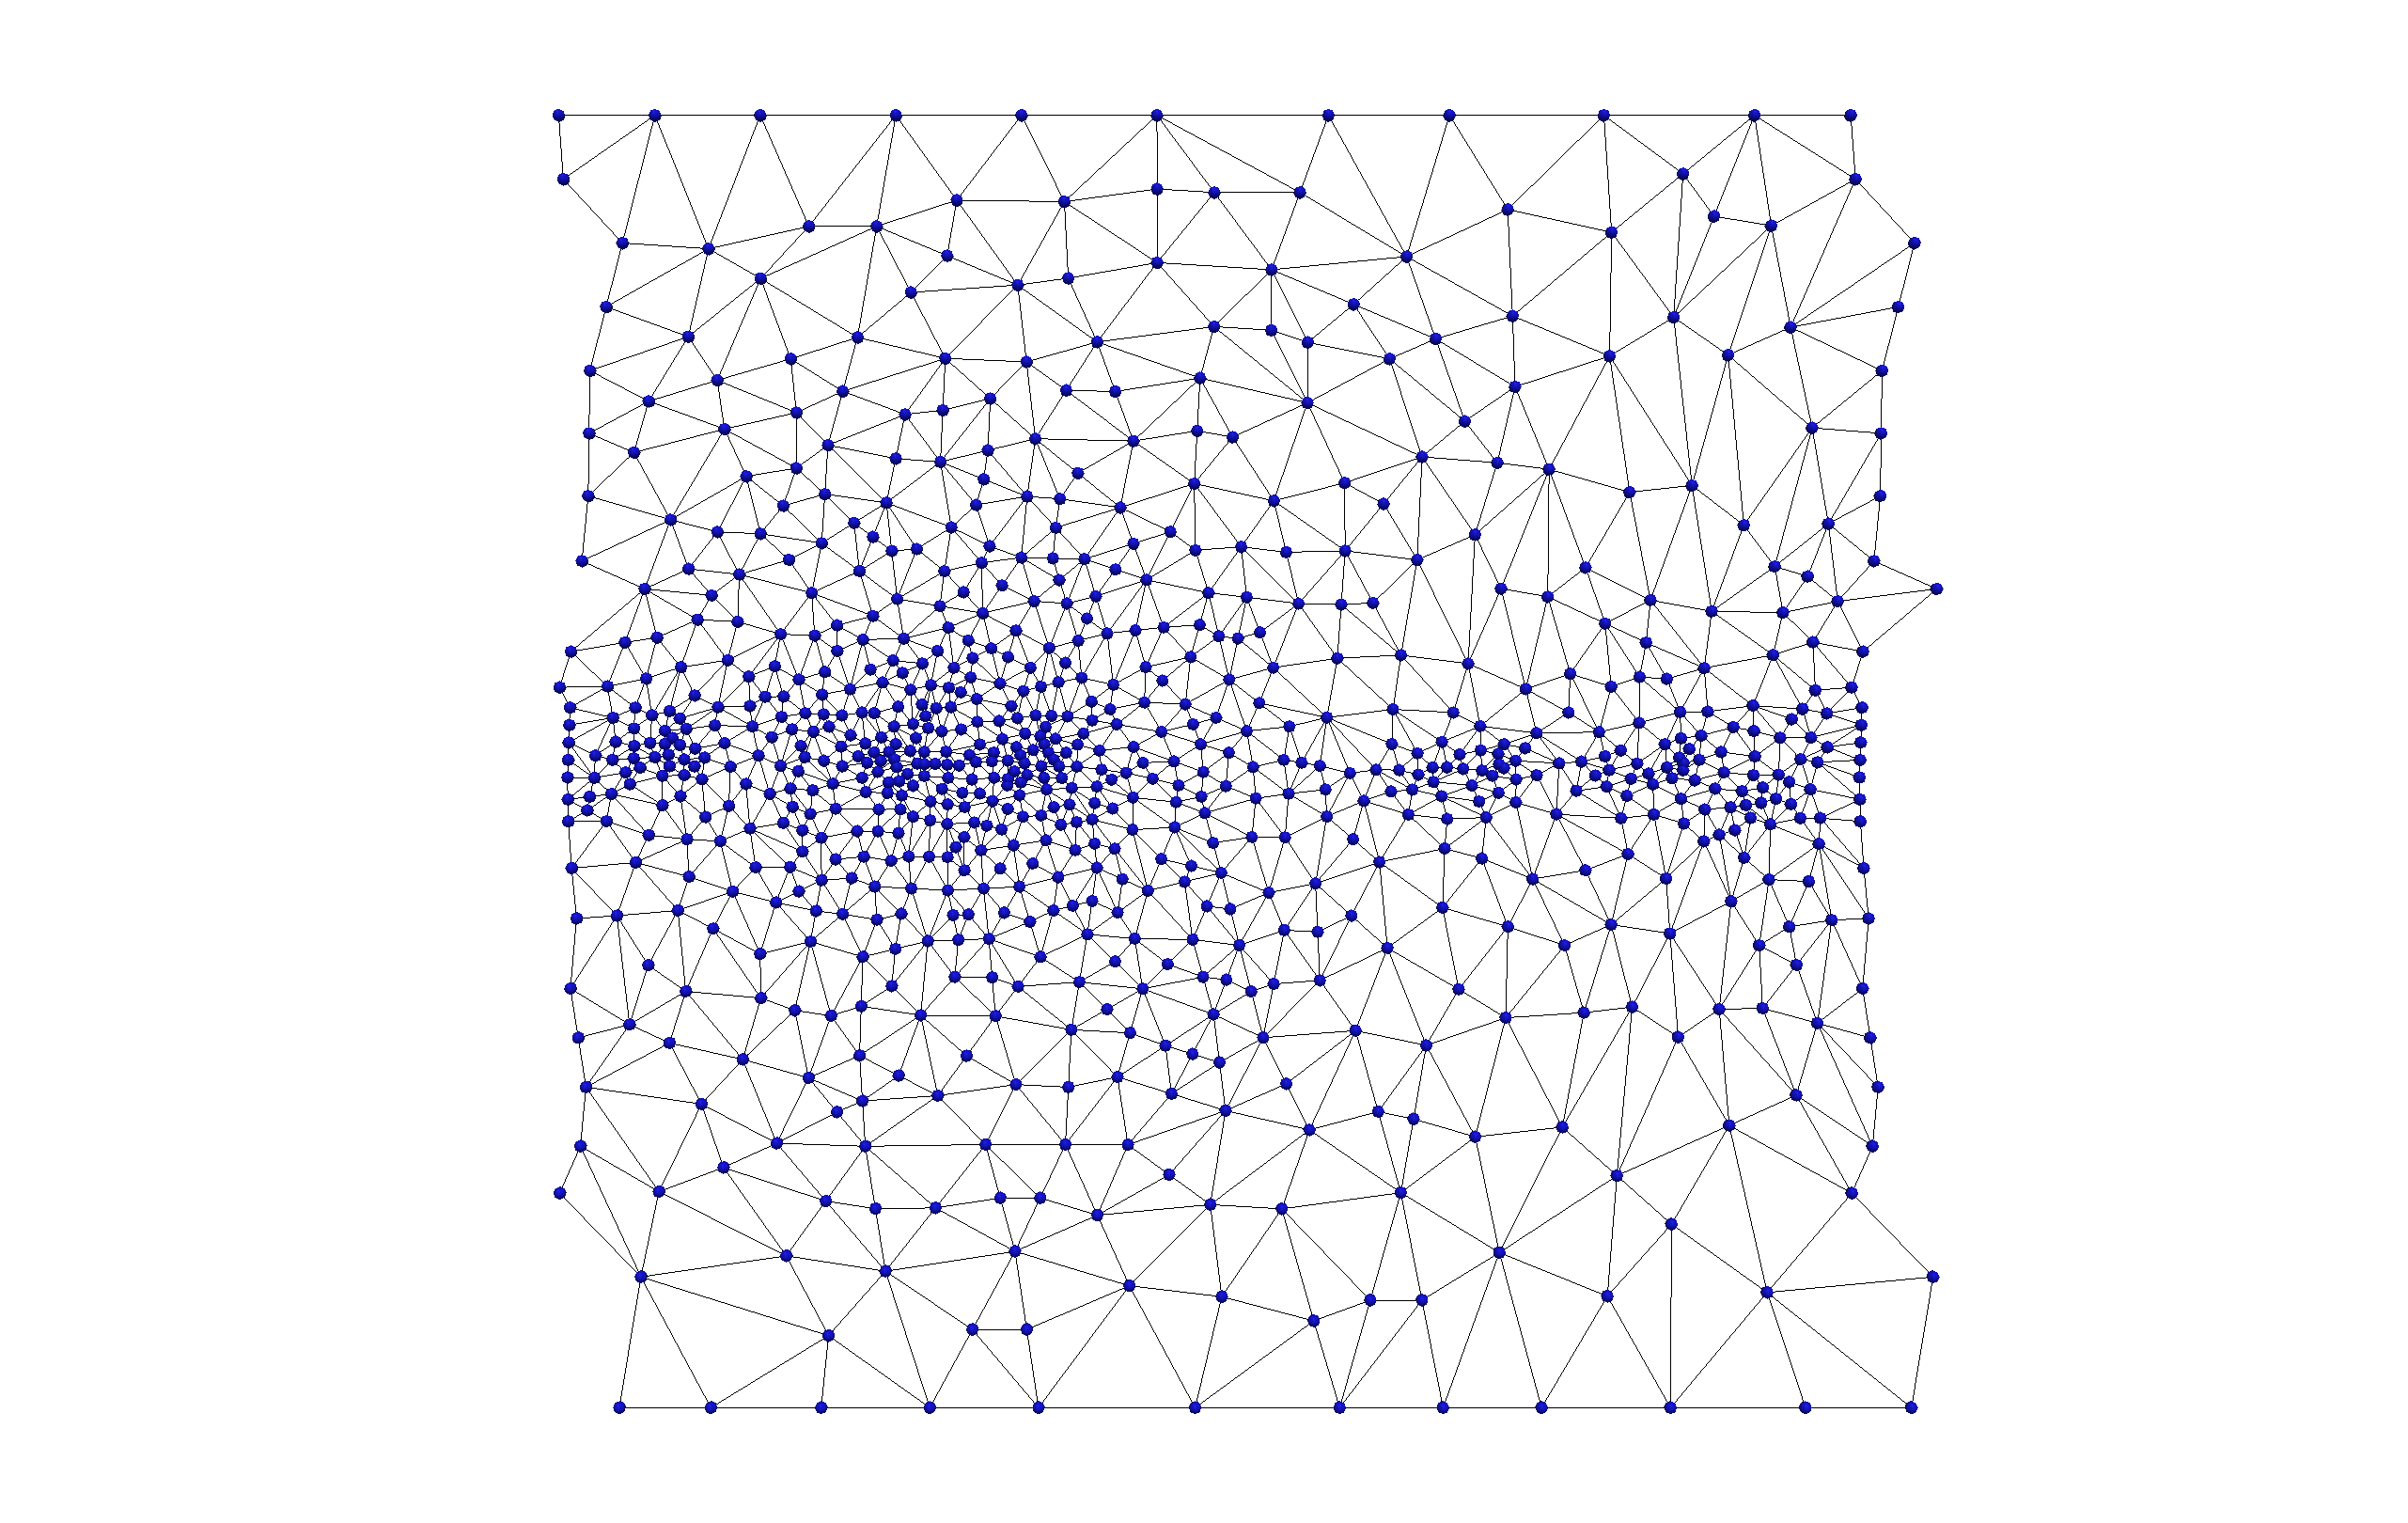
\includegraphics[width=0.9\textwidth]{periodic}

  \vspace{-1em}
  Periodic boundary conditions are implemented by identifying nodes on opposite
  sides of the periodic boundary. This leads to a new function space in which
  all solutions are automatically periodic.
\end{frame}

\begin{frame}{Source/Absorption}
  Two terms can be added to the advection diffusion equation:
  \begin{equation*}
    \ppt T + u\cdot\grad T - \kappa\nabla^2 T + \alpha T = s,
  \end{equation*}
  with absorption coefficient $\alpha$ and source $s$. Similarly, in the
  momentum equation
  \begin{equation*}
    \ppt{\vec u} + \vec u\cdot\grad\vec u - \nu\nabla^2\vec u
      + \grad P + \vec\sigma\cdot\vec u = \vec f,
    \end{equation*}
  with absorption vector $\vec\sigma$ and momentum source (force) $\vec f$.
\end{frame}

\begin{frame}{Sponge regions}
  Source and absorption terms can be used to define sponges in some regions. To relax to a value
  $T_r$, choose:
  \begin{equation*}
    s = \alpha T_r,\quad \alpha=1/\tau
  \end{equation*}
  where $\tau$ is the relaxation time. This relaxation time should be larger
  than your time step and smaller than the time scale of the dynamics you want
  to dampen out.
  
  Best to ramp up the value of $\alpha$ towards the sponge region
  to avoid reflections.
\end{frame}

\section{Linear solvers}
\begin{frame}{Linear solvers}
  \begin{block}{Computational methods to solver linear systems}
  \begin{itemize}
    \item Direct solvers. Only smallish problems (typically 2D)
    \item Iterative solvers - we use the PETSc library
  \end{itemize}
\end{block}

  For iterative solvers we need to choose:
  \begin{itemize}
    \item Krylov subspace method: CG or GMRES
    \item Preconditioners: SOR or MG (algebraic multigrid)
    \item Stopping criterion:
      \begin{itemize}
        \item relative:\;\; $r<C_{\text{rel}}~r_0$,
       \item absolute: $r<C_{\text{abs}}$,
      \end{itemize}
      where $r$ is the preconditioned residual.
    \item Maximum number of iterations.
  \end{itemize}

  {\small{\bf Overview iterative methods:} \citet{Saad1996}}
\end{frame}

\begin{frame}{Pressure solve options}
  The Pressure Poisson equation yields a symmetric positive definite matrix.
  This means we can use CG + SSOR (symmetric SOR=default). For bigger and more
  complex problems CG + MG is more efficient.

  \vspace{1em}
  For large aspect ratio problems, where the horizontal length scales are orders
  bigger than the vertical, use CG + MG +
  \lstinline{vertical_lumping}.\citep{Kramer2010}

  \vspace{1em}
  If all boundaries are closed (or have specified normal velocity)
  the pressure equation is not well-posed; We can add any constant to the
  solution. We need to tell this to the solver with \lstinline{remove_null_space}
  option.
\end{frame}

\begin{frame}{Momentum and scalar equations}
  Due to the advection term the matrices resulting from discretising the scalar
  advection-diffusion equation and the momentum equation are non-symmetric.
  Therefore we choose GMRES+SOR.

  \vspace{1em}
  High Courant numbers lead to high number of iterations or non-convergence.

  \vspace{1em}
  For pure diffusion equations (heat equation) CG+SOR/MG can be used.
\end{frame}

\section{References}
\begin{frame}{References}
  \tiny
  \bibliographystyle{plainnat}
  \bibliography{references}
  \normalsize Many more details and references in the Fluidity manual!
\end{frame}

\end{document}

